\documentclass{article}
%\usepackage[utf8]{inputenc}

%\documentclass[journal,12pt,onecolumn]{IEEEtran}
%\documentclass[10pt,peerreviewca]{IEEEtran}

\usepackage{geometry}
\geometry{ a4paper, total={170mm,257mm}, left=20mm, top=20mm }

\usepackage{caption}
\usepackage{listings}
\usepackage{enumerate}
\usepackage{comment}
\usepackage{algorithmic}
\usepackage{graphicx}
\usepackage{balance}
\usepackage{color}
\usepackage[caption=false]{subfig}

\usepackage{hyperref}
\hypersetup{colorlinks=true, linkcolor=blue, filecolor=magenta, urlcolor=cyan}

\linespread{1.2} % line spacing
\graphicspath{{./../Figs/}}

%%%%%%%
% Your paper was successfully submitted. Your paper is: hpcs17acidb 
% correct bad hyphenation here
\hyphenation{op-tical net-works semi-conduc-tor}

\begin{document}

\title{Predator-Prey Tutorial: Hands-on Practical Exercises}
\author{Mozhgan Kabiri Chimeh, Paul Richmond}
\date{}

% author names and affiliations
% use a multiple column layout for up to three different
% affiliations

%\author{\IEEEauthorblockN{Mozhgan Kabiri Chimeh\IEEEauthorrefmark{1}, Paul Richmond\IEEEauthorrefmark{2}}
%\IEEEauthorblockA{\IEEEauthorrefmark{1}\IEEEauthorrefmark{2}Department of Computing Science\\
%211 Portobello, University of Sheffield\\
%Sheffield, S1 4DP, UK}\thanks{Emails: m.kabiri-chimeh@sheffield.ac.uk, P.richmond@sheffield.ac.uk}}

%\markboth{Predator-Prey Tutorial: Hands-on Practical Exercises}{}


\maketitle

% To me: You may move this setting to the beginning of the document.
\lstset{numbers=none,
frame=none,
basicstyle=\ttfamily\footnotesize,
commentstyle=\scriptsize,
xleftmargin=2.2em,
columns=fullflexible,
breakatwhitespace=false,         
breaklines=true,                 
captionpos=b,                    
keepspaces=true,
numbersep=5pt,                  
showspaces=false,                
showstringspaces=false,
showtabs=false,                  
tabsize=2,
escapechar=\&}
%numbers=left,
%frame=leftline,
%numberstyle=\tiny,
%stepnumber=1,

\section{Introduction}

This document forms the hands-on practical component on how to use FLAMEGPU. You can download it from \href{www.flamegpu.com/tutorial}{www.flamegpu.com/tutorial}.

We will be using Amazon EC2 G2 Instances, optimised for graphics-intensive applications. To access this system, you have been provided with a username/password as well as a public domain name. 

Instructions for performing simulation and visualisation of models on an Amazon AWS GPU cloud instance will be provided as well as a sample models and data which will require completion of carefully defined step-by-step instructions. 

\textbf{Note:} If you have a laptop with CUDA-enabled GPU and have a CUDA 7.5 or CUDA 8.0 installed on it, feel free to skip Section~\ref{sec:aws}. However, it is expected for all attendees to use AWS as we do not offer assistance for setting up your machine.

\section{Predator-Prey model}
This section describes the FLAMEGPU implementation of a simple predator-prey model. The specification of the model is based on the previous implementations on FLAME~\cite{Poulter} and NetLogo~\cite{netlogo}. We briefly give an introduction to the FLAMEGPU software in Section~\ref{sec:flamegpu} followed by details of the predator-prey model in Section~\ref{sec:preypredator}. Section~\ref{sec:implementation} gives an overview of the various components of the FLAMEGPU implementation.

\subsection{FLAMEGPU framwork}\label{sec:flamegpu}
FLAME GPU (a template driven framework for Agent Based Modeling on parallel architecture) is an extended version of the FLAME (Flexible Large-scale Agent-based Modelling Environment) framework~\cite{Coakley2016} that enables modellers from various disciplines like economics, biology and social sciences to easily write agent-based models, specifically for Graphics Processing Units (GPUs).

For a  more detailed and comprehensive overview of the framework followed by an example, please refer to our full tutorial paper to be published in HPCS17~\footnote{FLAME GPU: Complex System Simulation Framework}

\subsection{Problem description}\label{sec:preypredator}
To begin with, we give a very general description of the predator-prey model in the NetLogo library without reference to its implementation. Then we will give more details on the
implementation before describing the FLAMEGPU version in the next section.

The predator-prey model has 2 versions. In the more basic form, there are prey
and predators which preys move in a groups and try to avoid predators, while predators are moving towards preys and this costs a predator some energy. If, after a particular move, a predator and prey are close enough (within a fixed radius), the predator is able to eat the prey and increase the amount of energy it has. Predators die when they run out of energy.

The second version of the model includes grass (i.e. food source for preys) as an additional component. If preys move to a location which has grass, they are able to eat. This increases the amount of energy they have, but they can no longer move for free, as similarly to predators, with each move, some energy is lost. Preys will now die either when they are eaten by a predator, or if they run out of energy.

When a prey eats grass, the grass in that area is set to re-grow after a set length of time. Both
predators and preys are able to reproduce with a fixed probability rate at each time step.


The model has been implemented in various frameworks (e.g:NetLogo and FLAME). The implementation in FLAMEGPU is based on following details:


\begin{itemize}
\item Predator and Prey agents move and act in a sequence of iterations.
\item Predator and Prey agents have an (x, y) position and velocity.
\item Predator agents have an initial speed. Predator's speed increases when is close to a prey/group of preys.
\item A predator’s energy is reduced by 1 unit each time it moves.
\item Predator agents can only eat prey agents within a fixed radius.
\item A predator’s energy increases each time it catches a prey
\item A predator dies if it has run out of energy.
\end{itemize}
Additionally, when grass or preys' source of food is included in the model~\footnote{based on NetLogo's implementation}:
\begin{itemize}
%\item Each grass is either "green" or "navy", indicating whether grass is currently there.
\item A prey’s energy is reduced by 1 unit each time it moves.
\item A prey’s energy increases each time it eats grass.
\item A prey dies if it has run out of energy.
\item Once eaten, grass regrows after a fixed number of iterations.
\end{itemize}

The details of the algorithms at the decision points are given below.

\paragraph{Prey catching}
There is no limit on the amount of preys, a predator can eat per iteration. If there are multiple preys within the specific radius, predator can kill/eat them all. Moreover, a prey cannot be shared between multiple predators. If there are multiple predators and 1 prey within the killing distance, the first predator to attempt to catch the prey will do so.

\paragraph{Reproduction}
There is a set value for reproduction that can be different for predator and prey. At every iteration, we draw a random floating number between 0 to 1. If this number is less than the set value for reproduction then a new agent is created. The parent’s energy is shared with the new agent, so both will have half of the parent’s energy for the next iteration.

\subsection{FLAMEGPU implementation}\label{sec:implementation}
We designed the model based and implement the agent functions based on the assumption made in previous section. All agents have a position (x, y) in the domain as well as velocity. Moreover, predator agents also have an initial speed. In the basic model, only the predator agents have a variable (\verb|life|) which contains the amount of energy each have. However, in the second version of the model, in addition to the predators, prey agents also have a \verb|life| variable indicating the amount of energy they have.

In the case of implementing the second variant of the predator-prey model, grass agents have a boolean flag \verb|available| indicating whether there is currently grass at their location.

Moreover, unique ids are required for the predators and preys. When a predator kills a prey, it is necessary to know the id of both as this will be explained later in this section.

All communication between agents in FLAMEGPU is done via messages and in this model we have 3 messages ,or 5 when grass is included. The mechanism for "killing" is as follows:

\begin{enumerate}
\item Both prey and predator output their (x, y) coordinates to a location message.
\item Preys avoid predators
\item Predators read preys locations and move towards them
\item Prey read each others location and move towards each other producing flocking behaviour.
\item Predators read each others location and try to avoid each other by changing directions.
\item Prey reads locations of predators and if there was a predator in close enough proximity, then it outputs the \verb|prey_eaten_message| message and dies.
\item Predator read the \verb|prey_eaten_message| message and checks the id against its id. If the message indicates that the predator ate some prey, then increases its energy/life accordingly.
\end{enumerate}

When grass is included in the model a fourth and fifth message is required as a prey can only eat grass within a certain radius. The mechanism for "grazing" is as follows:

\begin{enumerate}
\item  Grass agents which currently have grass read the positions of the prey from the location
message.
\item  Grass agents read the positions of the prey from the location message. Then, each pick out the messages within the minimum distance and then post the ID of a prey within that distance to the \verb|grass_eaten_message| message. Note that if there is more than 1 prey on within the minimum distance, the grass agent will be eaten by the closest prey.
\item  Grass agents then modify the boolean flag to indicate they no longer have grass at this
time. The colour also changes from "green" to "navy".
\item  Prey agents read the \verb|grass_eaten_message| message which contain their ID. They then increase their energy accordingly.
\item Prey agents die if they dont' have enough life/energy
\end{enumerate}

\subsection{The FLAMEGPU Model}
Various elements of the FLAMEGPU model is as below:
\begin{itemize}
    \item \textbf{environment} - holds global information related to the simulation such as constant variables, C code file name
\item \textbf{agents} - all things related to the agents
\item \textbf{messages} - represent information which is communicated between agents
\end{itemize}

To download the predator-prey \verb|XMLModelFile.xml|, follow the instructions given in Section~\ref{sec:hands-on}. Various tags have been used to define the model. Please refer to the FLAMEGPU user manual for detail~\cite{richmond11b}.
\subsubsection{FLAMEGPU environment}
The environment section contains various user defined constants and specific functions. For the Predator-Prey model, some of the parameters that define the behaviour of the agents are included in the environment section. 
\begin{verbatim}
<gpu:environment>
    <gpu:constants>
        <gpu:variable>
            <type>float</type>
            <name>REPRODUCE_PREY_PROB</name>
            <defaultValue>0.03</defaultValue>
        </gpu:variable>
        <gpu:variable>
            <type>float</type>
            <name>REPRODUCE_PREDATOR_PROB</name>
            <defaultValue>0.03</defaultValue>
        </gpu:variable> 
        <gpu:variable>
            <type>int</type>
            <name>GAIN_FROM_FOOD_PREDATOR</name>
            <defaultValue>15</defaultValue>
        </gpu:variable>
        <gpu:variable>
            <type>int</type>
            <name>GAIN_FROM_FOOD_PREY</name>
            <defaultValue>5</defaultValue>
        </gpu:variable>
    </gpu:constants>
    <gpu:functionFiles>
        <file>functions.c</file>
    </gpu:functionFiles>
    <gpu:initFunctions>
        <gpu:initFunction>
            <gpu:name>initLogFile</gpu:name>
        </gpu:initFunction>
    </gpu:initFunctions
    <gpu:exitFunctions>
        <gpu:exitFunction>
            <gpu:name>closeLogFile</gpu:name>
        </gpu:exitFunction>
    </gpu:exitFunctions>
    <gpu:stepFunctions>
        <gpu:stepFunction>
            <gpu:name>outputToLogFile</gpu:name>
        </gpu:stepFunction>
    </gpu:stepFunctions>
</gpu:environment>
\end{verbatim}
\subsubsection{Agent memory}
The agent definition is tagged by \verb|<xagents>|. Agent memory variables are defined in this section. Below is an examples of "grass" agent memory containing multiple agent variables:

\begin{verbatim}
<memory>
    <gpu:variable>
        <type>int</type>
        <name>id</name>
    </gpu:variable>
    <gpu:variable>
        <type>float</type>
        <name>x</name>
    </gpu:variable>
    <gpu:variable>
        <type>float</type>
        <name>y</name>
    </gpu:variable>
    <gpu:variable>
        <type>float</type>
        <name>type</name>
    </gpu:variable>
    <gpu:variable>
        <type>int</type>
        <name>level</name>            
    </gpu:variable>
    <gpu:variable>
        <type>int</type>
        <name>available</name>            
    </gpu:variable>
</memory> 
\end{verbatim}



\subsubsection{Agent functions} % Func description from Paul's Tutorial @ Rabat
The Functions aspect of the agent description describes the properties of the behaviours that the agent will have. Note: This is not where the actual behaviour is described but the properties relating to the behaviour functions. Table~\ref{tab:1} and Table~\ref{tab:2}, shows the list of defined functions per agent in the predator-prey model. 


\begin{table}[h]
\centering
\caption{Summary of the Prey agent functions for Predator Prey model - no grass included}
\begin{tabular}{ |l|l| } 
\hline
Function & Description\\
\hline\hline
prey\_output\_location& each prey agent outputs information to be read by other agents\\\hline
prey\_avoid\_pred& prey agents avoiding predator agents\\\hline
prey\_flock& flocking between prey agents\\\hline
prey\_move & movement of prey agents\\\hline
prey\_eaten & prey agents get killed by predator agents\\\hline
prey\_eat\_or\_starve & prey agents gain energy or starve (only when grass included in the model)\\\hline
prey\_reproduction & regeneration of preys\\
\hline
\end{tabular}
\label{tab:1}
\end{table}

\begin{table}[h]
\centering
\caption{Summary of the Predator agent functions for Predator Prey model - no grass included}
\begin{tabular}{ |l|l| } 
\hline
Function & Description\\
\hline\hline
pred\_output\_location& each predator agent outputs information to be read by other agents\\\hline
pred\_follow\_prey& predator agents follow prey agents\\\hline
pred\_avoid& predator agents avoid each other\\\hline
pred\_move & movement of predator agents\\\hline
pred\_eat\_or\_starve & predator agents gain energy or starve\\\hline
prey\_reproduction & regeneration of predators\\
\hline
\end{tabular}
\label{tab:2}
\end{table}



Functions are applied to agents in a specified initial\_state and will result in the agent moving into a next\_state (or the same state). Furthermore, functions can have conditions. For example, a function which simulates agent death might check a variable incremented each iteration called life-cycles to see if it has reached a maximum number. Only agents meeting this condition would perform the behaviour and move into a dead state.  The predator-prey model is a fairly simple model and does not have any function conditions.

Functions can have either a single input or output (or neither). Inputs and outputs are in the form of messages which are a collection of variables which are persistent from the point in which they are output to the end of the simulation iteration (at which point they are destroyed).  A function description within a model requires that any inputs or outputs are fully specified. 



Listing~\ref{lst:XML_output_func} shows the structure of a Function description in a model. In this example, the agent function has a message output which updates the agents internal memory. In order to add a new agent function, simply add the the XML code to the model after the existing function definitions.


\begin{lstlisting}[linewidth=\columnwidth,breaklines=true,language=C++,caption={},label=lst:XML_output_func]
<gpu:function>
    <name>prey_output_location</name>
    <currentState>default1</currentState>
    <nextState>default1</nextState>
    <outputs>
        <gpu:output>
            <messageName>prey_location</messageName>
            <gpu:type>single_message</gpu:type>
        </gpu:output>
    </outputs>
    <gpu:reallocate>false</gpu:reallocate>
    <gpu:RNG>false</gpu:RNG>
</gpu:function>
\end{lstlisting}

The additional reallocate and \verb|RNG| tags are used to specify if the agent function may result in agent death (reallocate) or if a random number generator is required (RNG). 

Note that for each message type defined within the XMML model definition, the dynamically generated simulation API will create a message output function. Agents can only output a single message per agent function. In Listing~\ref{lst:output_func}, agent prey outputs a message with three variables.

\begin{lstlisting}[linewidth=\columnwidth,breaklines=true,language=C++,caption={},label=lst:output_func]
__FLAME_GPU_FUNC__ int pred_output_location(xmachine_memory_predator* xmemory, xmachine_message_pred_location_list* pred_location_messages)
{
	add_pred_location_message(pred_location_messages, xmemory->id, xmemory->x, xmemory->y);
	return 0;
}
\end{lstlisting}

Moreover, iterating over message input (message list) within agent function is also possible by the use of dynamically generated message API functions. Listing~\ref{lst:eaten_func} shows a complete agent function with input messages demonstrating the iteration of a message list and outputting a different message. The while loop (\verb|while (pred_location_message)|) continues until the \verb|get_next_pred_location_message| return a NULL or a false value. 


\begin{lstlisting}[linewidth=\columnwidth,breaklines=true,language=C++,caption={},label=lst:eaten_func]
__FLAME_GPU_FUNC__ int prey_eaten(xmachine_memory_prey* xmemory, xmachine_message_pred_location_list* pred_location_messages, xmachine_message_prey_eaten_list* prey_eaten_messages)
{
	int eaten = 0;
	int predator_id = -1;
	float closest_pred = PRED_KILL_DISTANCE;

	//Iterate the predator location messages until NULL is returned which indicates all messages have been read.
	xmachine_message_pred_location* pred_location_message = get_first_pred_location_message(pred_location_messages);
    while (pred_location_message)
	{
		//calculate distance between prey and predator
		float2 predator_pos = float2(pred_location_message->x, pred_location_message->y);
		float2 prey_pos = float2(xmemory->x, xmemory->y);
		float distance = length(predator_pos - prey_pos);

		//if distance is closer than nearest predator so far then select this predator as the one which will eat the prey
		if (distance < closest_pred)
		{
			predator_id = pred_location_message->id;
			closest_pred = distance;
			eaten = 1;
		}

		pred_location_message = get_next_pred_location_message(pred_location_message, pred_location_messages);
	}

	//if one or more predators were within killing distance then notify the nearest predator that it has eaten this prey via a prey eaten message.
	if (eaten)
		add_prey_eaten_message(prey_eaten_messages, predator_id);

	//return eaten value to remove dead (eaten == 1) agents from the simulation
	return eaten;
}
\end{lstlisting}


After adding the function definition to the XML model file, the new function should be added to the layers. Layers represent synchronisation points in the execution of the agent functions. It is assumed that functions on the same layer execute simultaneously so functions which have a dependency via messages should not be within the same layer. The \verb|prey_output_location|, \verb|prey_follow_prey| and \verb|prey_flock| functions are in different layers for this reason. 

In the case of \verb|prey_output_location| function, it will be added to the layer so that it executes in the same layer as \verb|pred_output_location|. The other functions are are added after the output location function to ensure they begins executing after all prey agents have completed outputting each prey's location (Listing~\ref{lst:XML_layer}).

\begin{lstlisting}[linewidth=\columnwidth,breaklines=true,language=C++,caption={},label=lst:XML_layer]
<layer>
    <gpu:layerFunction>
        <name>prey_output_location</name>
    </gpu:layerFunction>
    <gpu:layerFunction>
        <name>pred_output_location</name>
    </gpu:layerFunction>
</layer>
<layer>
    <gpu:layerFunction>
        <name>prey_flock</name>
	</gpu:layerFunction>
	<gpu:layerFunction>
        <name>pred_avoid</name>
	</gpu:layerFunction>
</layer>
<layer>
...
</layer>
\end{lstlisting}



\subsubsection{Agent messages}
All the agent communication is done via messages. In the second version of the model with grass included, we have five different message types: \textit{predator\_location}, \textit{prey\_location},\textit{grass\_location}, \textit{prey\_eaten}, \textit{grass\_eaten}. These messages contain all the required information by other agents in order to interact with each other. The description of \verb|grass_location| message is as below:
\begin{verbatim}
<messages>
    <gpu:message>
        <name>grass_location</name>
        <description>a message holding the location of an agent</description>
        <variables>
            <gpu:variable>
               <type>int</type>
               <name>id</name>
            </gpu:variable>
            <gpu:variable>
               <type>float</type>
               <name>x</name>
            </gpu:variable>
            <gpu:variable>
               <type>float</type>
               <name>y</name>
            </gpu:variable>
        </variables>
        <gpu:partitioningNone/>
        <gpu:bufferSize>262144</gpu:bufferSize>
    </gpu:message>
..
<messages>
\end{verbatim}

To download the complete XML model file for both versions of the model, follow the instructions given in Section~\ref{sec:hands-on}.

\subsection{The FLAMEGPU flow diagram}
Figure~\ref{fig:flowdiagram1} and Figure~\ref{fig:flowdiagram2} shows the dependency graph for the Predator-Prey model with and without grass implementation.

\begin{figure}[h]
    \centering
    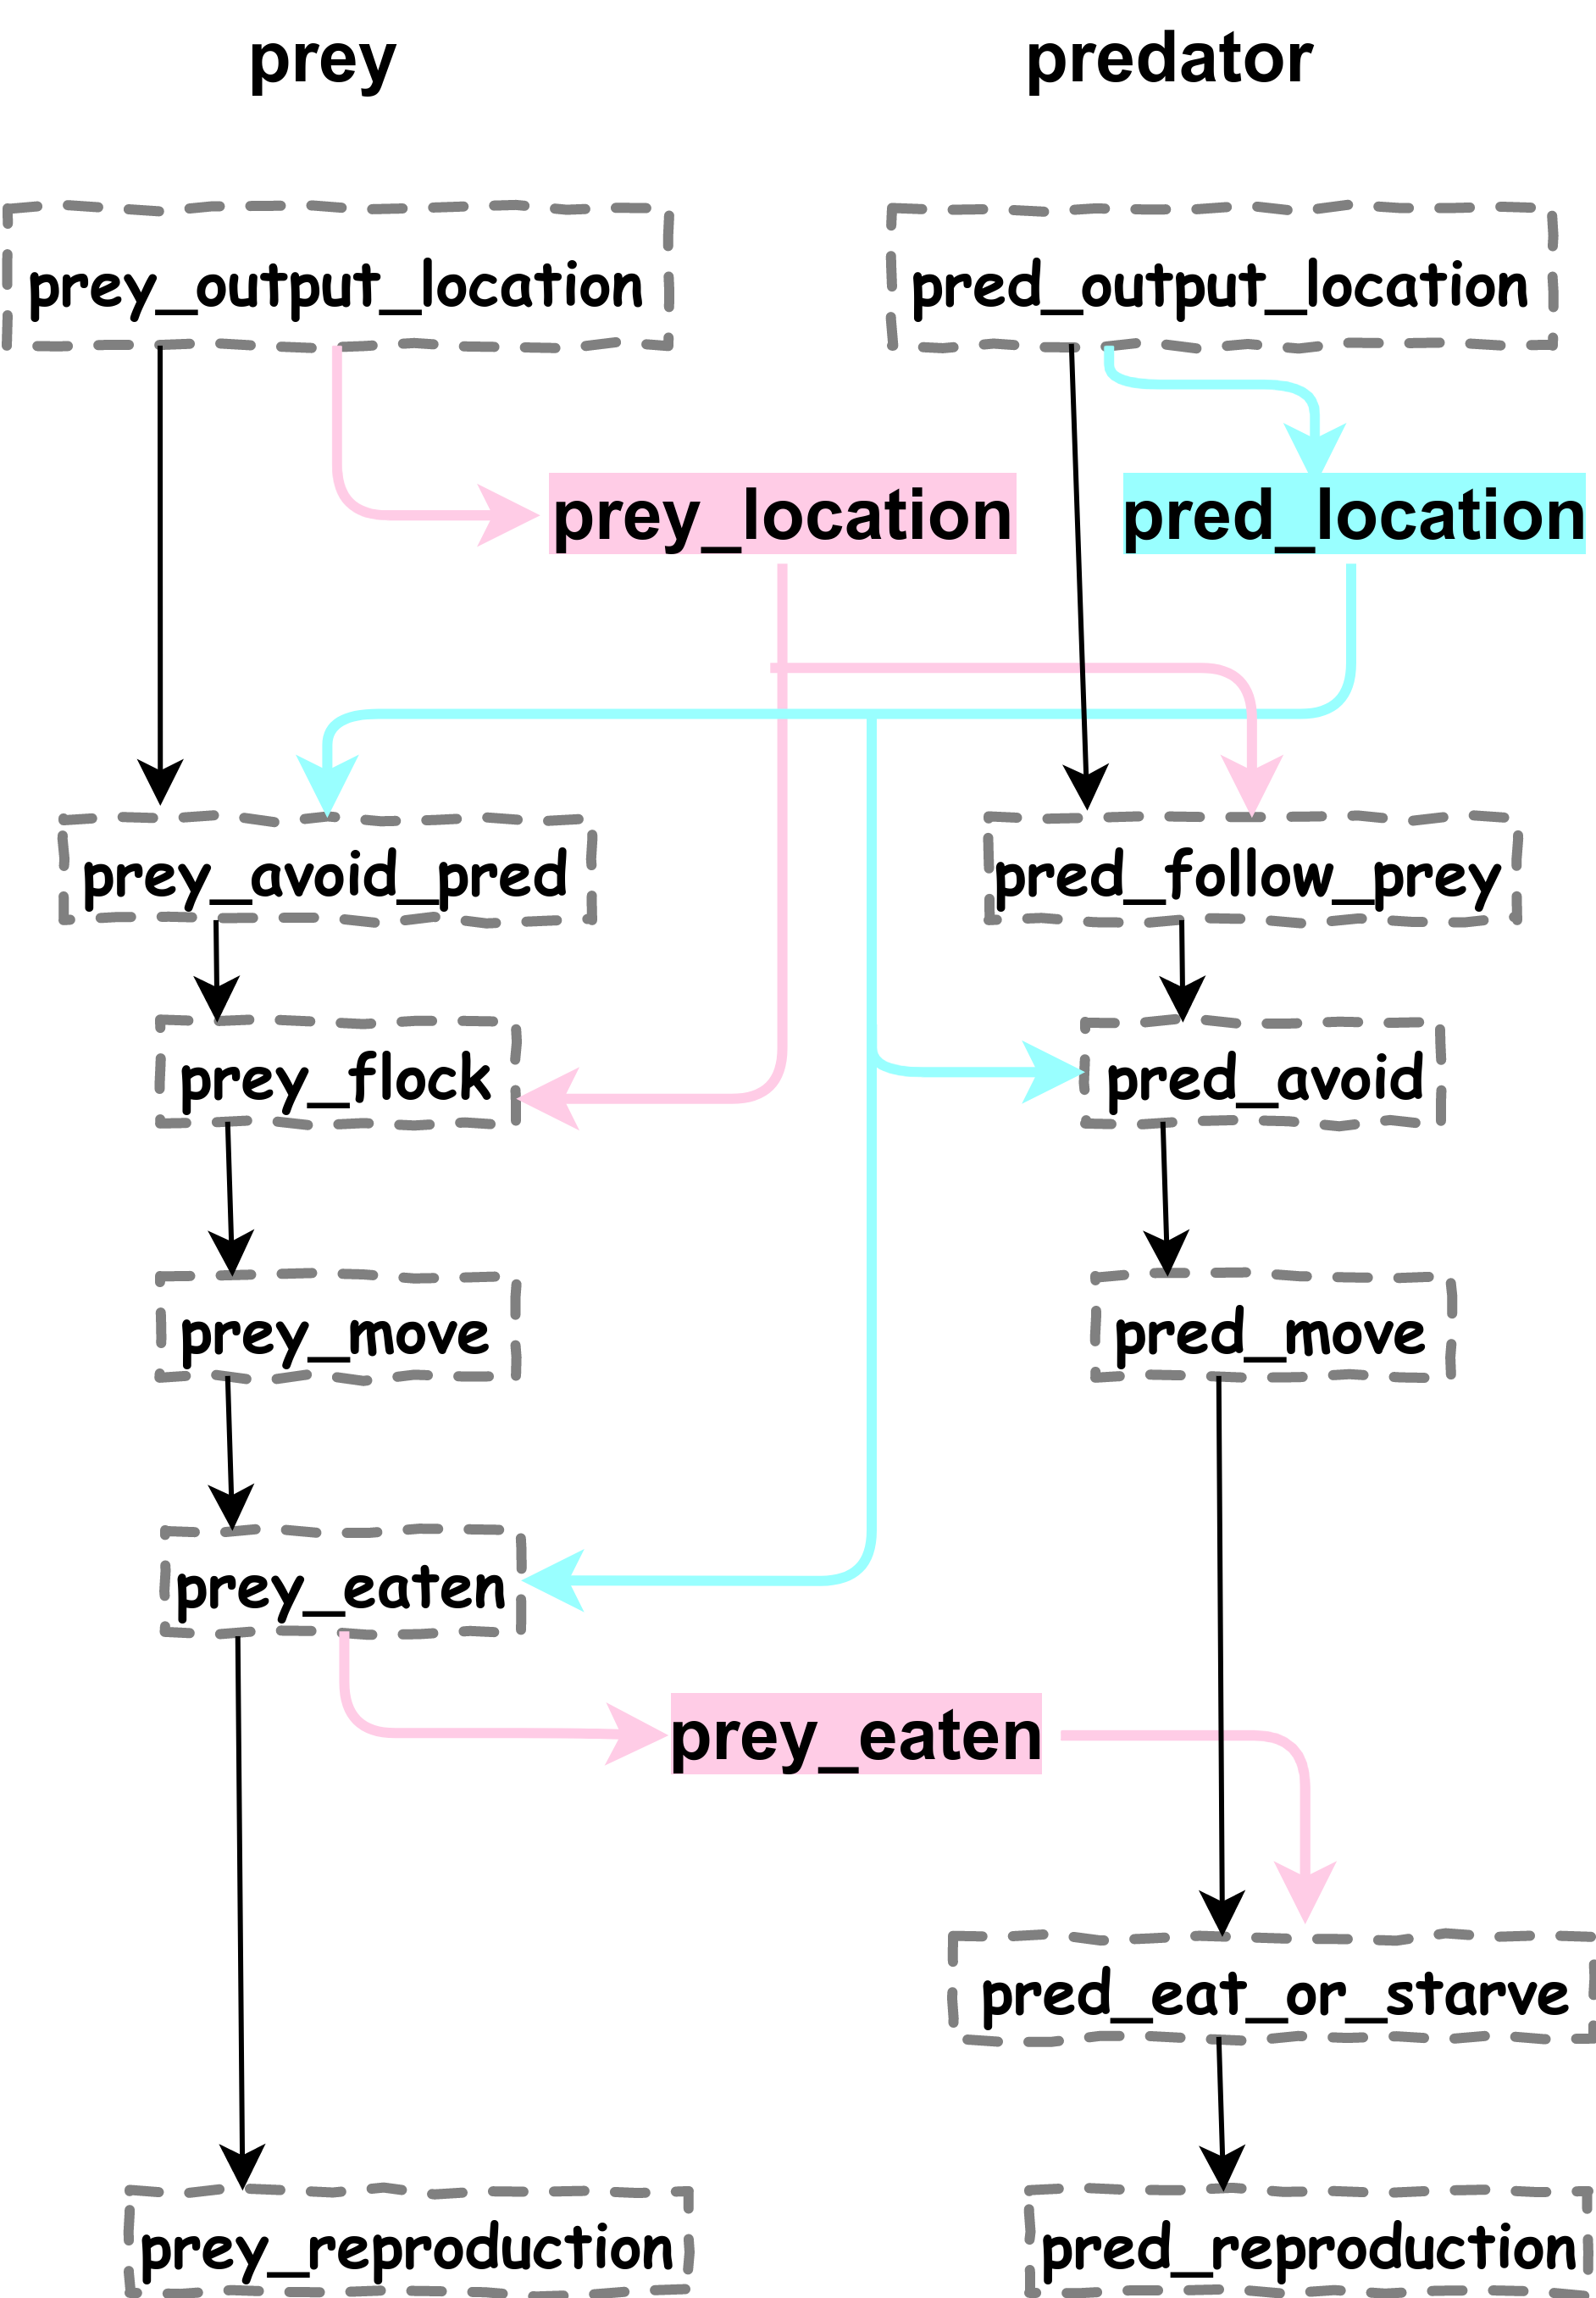
\includegraphics[width=3.2in]{prey_pred}
    \caption{Flow diagram for Predator-Prey model without grass}
    \label{fig:flowdiagram1}
\end{figure}

\begin{figure}[h]
    \centering
    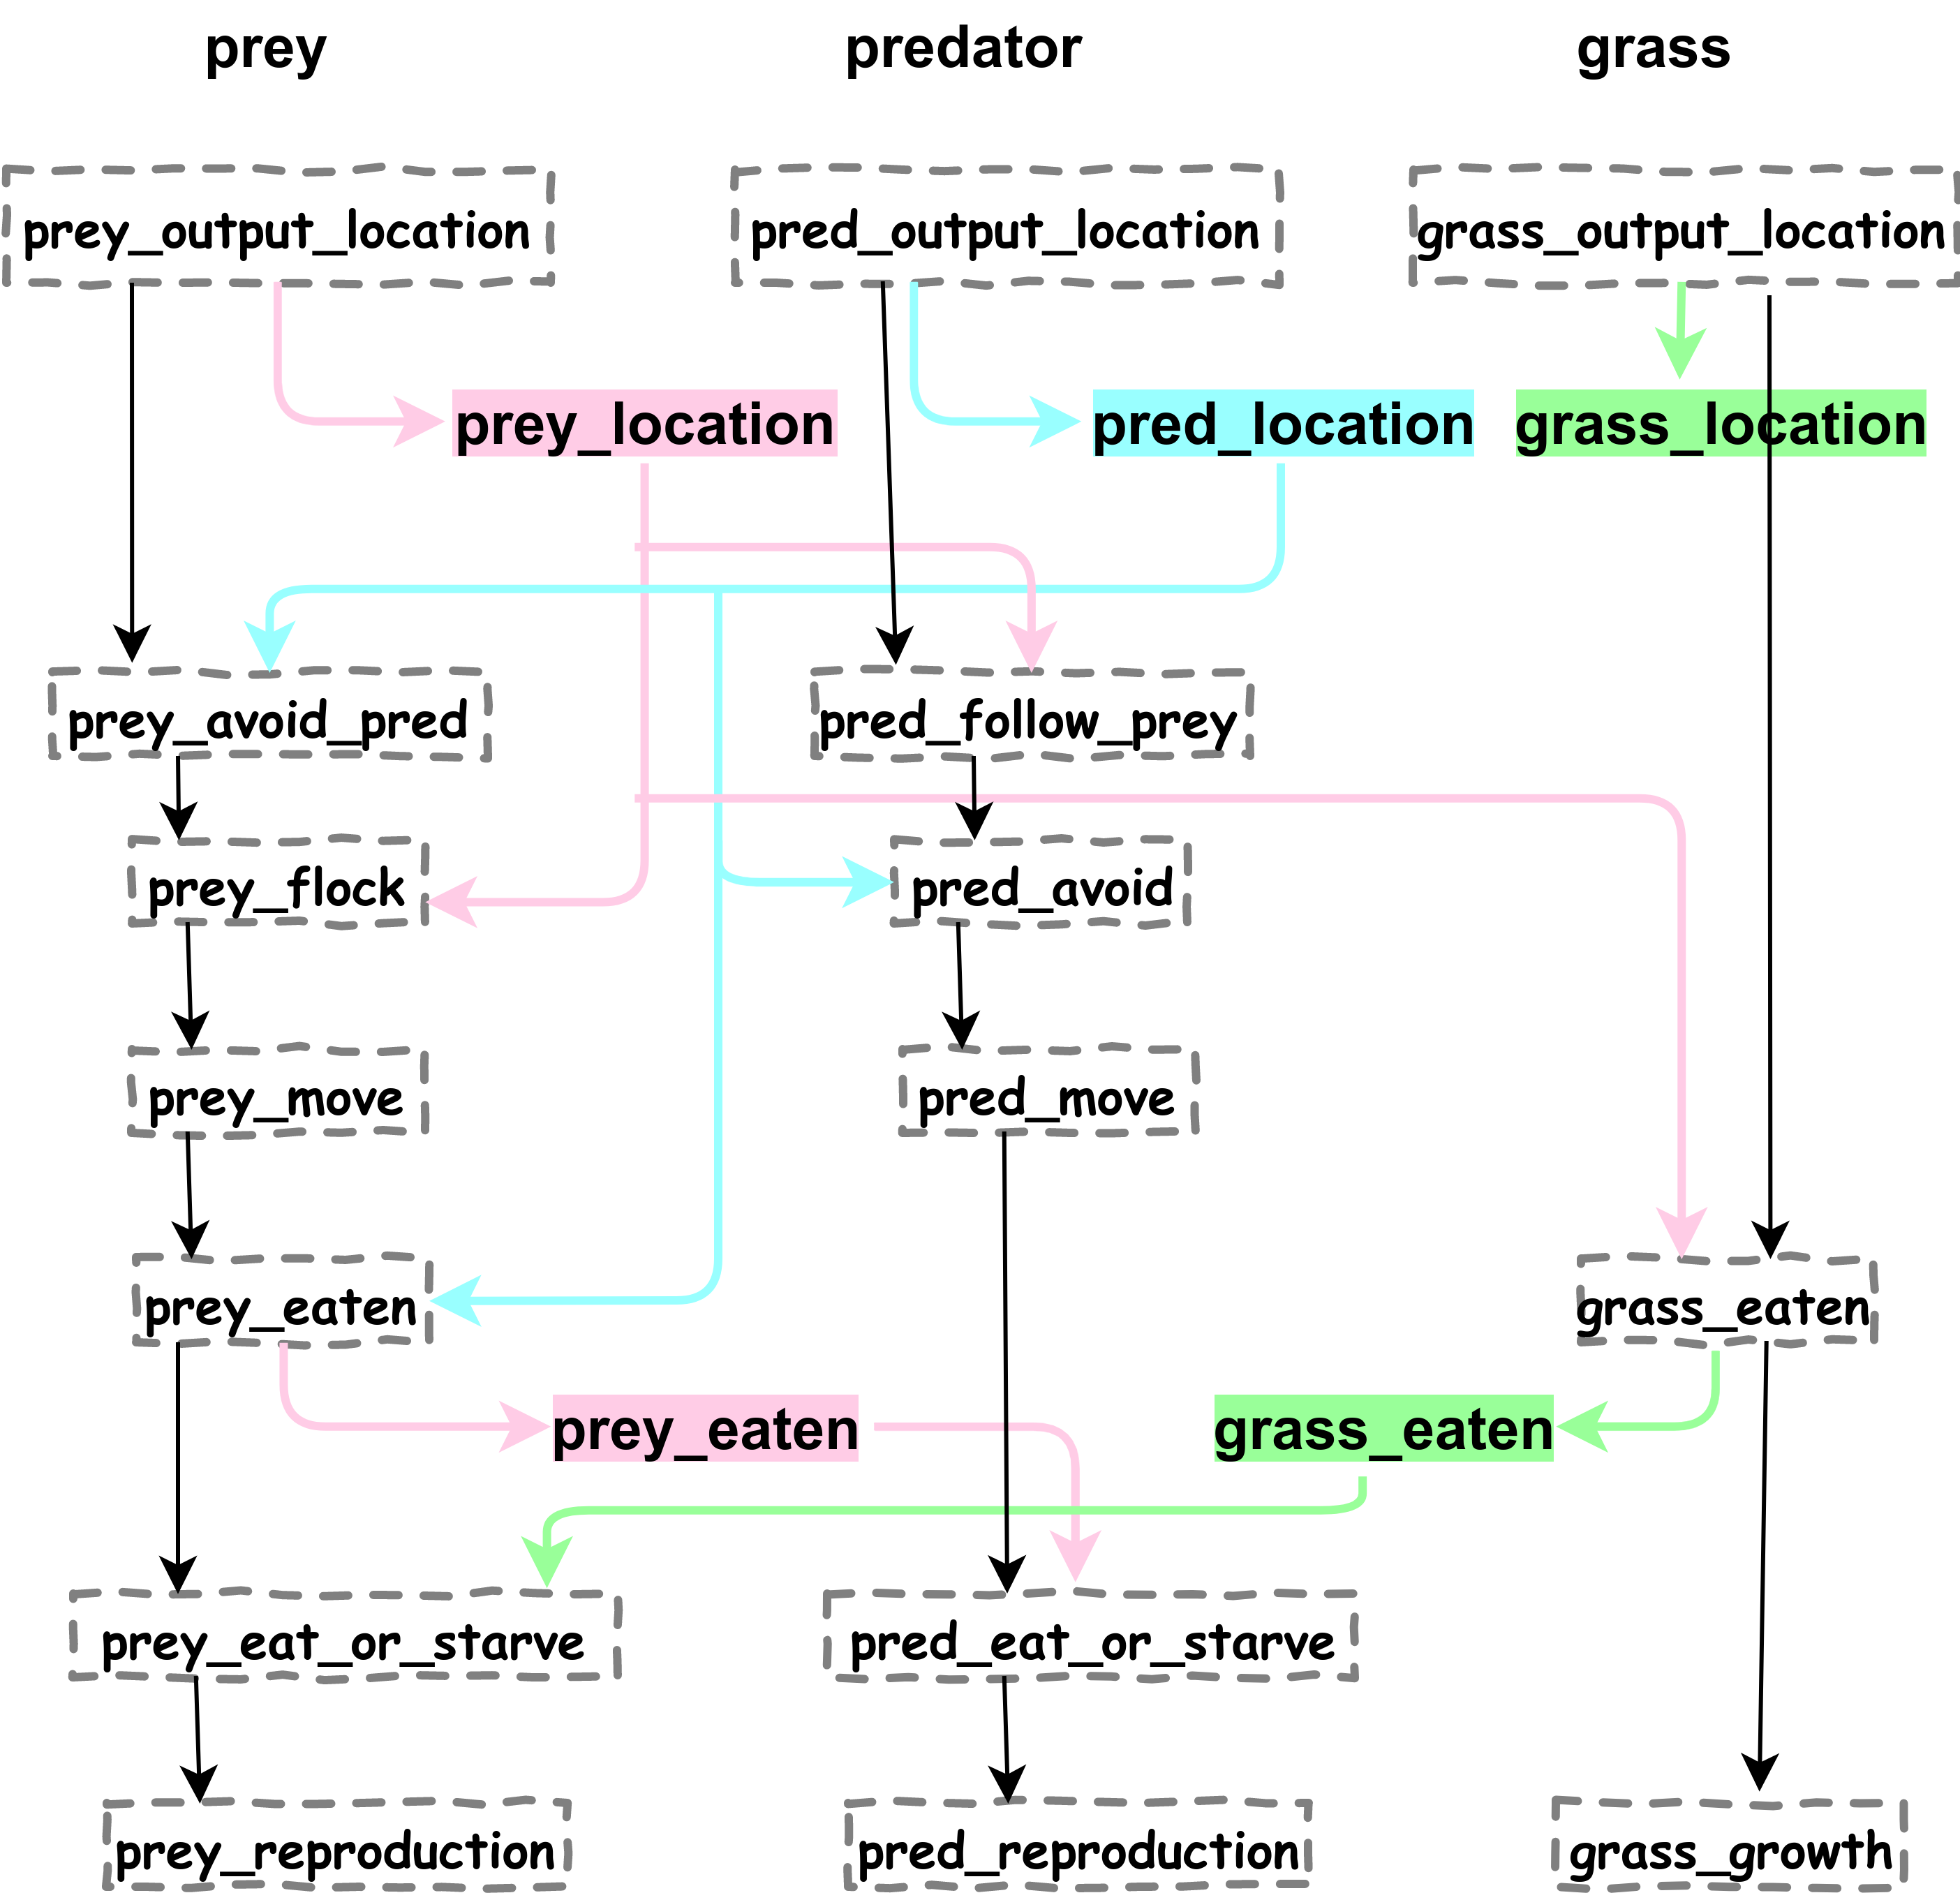
\includegraphics[width=4.2in]{prey_pred_grass}
    \caption{Flow diagram for Predator-Prey model with grass}
    \label{fig:flowdiagram2}
\end{figure}

\clearpage
\subsection{Input data generation and Setup}
The initial data for the model is generated using a simple c++ program. The program generates the specified number of predator and prey agents in random positions (\verb|x,y|) between [-1,1] with random velocities (\verb|fx,fy|) between [-1,1]. Moreover, each predator is given an amount of energy (\verb|life|) which is randomly selected from the interval of [0,40]. This interval is chosen to align the initial data close to the FLAME and NetLogo implementation. 

In the case where grass in included, prey agents require an energy (\verb|life|) variable similar to predators. This variable is randomly selected from the interval of [0,50]. The grass agent initial colour is set to "green". Once eaten, the \verb|available| variable is set to 0 and it takes upto \verb|GRASS_REGROW_CYCLES| iterations till the grass re-grow. 

The program generates an \verb|0.xml| output file containing the initial data. Table~\ref{tab:param} shows the various parameters used for the implementation of the model in FLAMEGPU.

\begin{table}[h]
\centering
\caption{Summary of parameters in Predator Prey model - grass included}
\begin{tabular}{ |l|l| } 
\hline
Parameter & Value \\
\hline\hline
Initial number of prey agents & 800\\\hline
Initial number of predator agents & 400\\\hline
Initial number of grass agents & 2000\\\hline
Amount of energy gained from eating prey & 75\\\hline
Amount of energy gained from eating grass & 50\\\hline
Probability of predators reproducing & 0.03\\\hline
Probability of preys reproducing & 0.05\\\hline
Number of iterations before grass can re-grow & 100\\
\hline
\end{tabular}
\label{tab:param}
\end{table}


\newpage
\section{Connecting to the Linux Instance}\label{sec:aws}
To get started with FLAMEGPU tutorial, you first need to connect to the AWS G2 instances. These are optimised for graphics-intensive application\footnote{Each GPU has 1,536 CUDA cores}. We have previously installed Ubuntu 16.04 and other required applications.

\subsection{Using SSH in Linux}
Connect to the Linux Instance using SSH command and the provided username\/password. Replace the \textit{public\_dns\_name} with the ones given to you by the instructors.

\begin{verbatim}
ssh username@public_dns_name
\end{verbatim}

\subsection{Using SSH in PuTTY}
\begin{enumerate}
     \item Putty is a free software application and can be downloaded from \href{https://www.chiark.greenend.org.uk/~sgtatham/putty/}{https://www.chiark.greenend.org.uk/~sgtatham/putty/} and run putty.exe
     \item In the Category pane, select Session and complete the following fields:

\begin{itemize}
\item In the Host Name box, enter \verb|username@public_dns_name|.
\item Under Connection type, select SSH.
\item Ensure that Port is 22.
\end{itemize}

\begin{figure}[!t]
    \centering
   % \includegraphics[width=3in]{putty} %putty
    %\caption{}
    \label{fig:putty}
\end{figure}
\item (Optional) If you plan to start this session again later, you can save the session information for future use. Select Session in the Category tree, enter a name for the session in Saved Sessions, and then choose Save.

\item Choose Open to start the PuTTY session

\item If this is the first time you have connected to this instance, PuTTY displays a security alert dialog box that asks whether you trust the host you are connecting to. 

\item Choose Yes. A window opens and a terminal prompt asking for your username:
\verb|login as:|
Enter your username.
\item Enter your password and you are connected to the instance. 
\end{enumerate}
   
\subsection{Transferring files}
Linux users can transfer files from your computer to the \verb|username| home directory via \verb|SCP| command.
\begin{verbatim}
scp /path/yourfile.txt username@dns_name:~
\end{verbatim}

Windows users can use the PuTTY Secure Copy client (PSCP) (a command-line tool) to transfer files between Windows computer and the Linux instance. 

\begin{verbatim}
pscp C:\path\yourfile.txt username@public_dns:/home/username/yourfile.txt
\end{verbatim}

\subsection{Display images via SSH}\label{sec:visualisation}
In order to view images, we will need to configure X11 window forwarding so that the OpenGL windows is opened on our local machine. If you are using Linux as your host operating system then you do not need to install anything. If you are using Windows you will need to install an X11 window server so that the remote machine where we are executing FLAME GPU can display on your local machine. The XMing software is free and is recommended. 
You should disconnect your SSH session to the AWS image and connect again making sure to enable X11 forwarding. From the command line, this requires that you use the ssh –X option. From Putty in Windows, this can be enabled from the Connection-SSH-X11 dialogue.
\newpage
\section{Getting started with FLAMEGPU}\label{sec:hands-on}

To get started with FLAMEGPU, connect to the Amazon instance by following the given instructions in Section~\ref{sec:aws}. Then, download the latest version of FLAMEGPU from GitHub:

%git clone https://github.com/FLAMEGPU/FLAMEGPU.git
\begin{verbatim}
git clone https://github.com/FLAMEGPU/Tutorial.git
\end{verbatim}


A typical top-level directory layout is as below:
%The folder structure of FLAMEGPU is as follows:

\begin{itemize}
\item \textbf{FLAMEGPU:} contains the templates and XML schemas that are used to generate CUDA GPU code. These should not be modified by the users.
\item \textbf{bin/x64} and \textbf{bin/linux-x64:} The location of the console and visualisation binaries for each of the examples. There is a Linux shell script for each example which will start the simulation with an initial states file (and the number of iterations to simulation in console mode)
\item \textbf{doc:} The FLAMEGPU technical report and user guide in addition to reports for specific example models.
\item \textbf{examples:} The location of the model files for FLAMEGPU examples and the location to create your own models.
\item \textbf{include:} Some common include files required by FLAMEGPU
\item \textbf{lib:} Any library dependencies required by FLAMEGPU
\item \textbf{media:} 3D models used for some of the visualisations
\item \textbf{tools:} A number of tools for generating function script files from XML model files and running template code generation in windows.
\end{itemize}

To start with, we are going to work with the predator-prey model (Section~\ref{sec:preypredator}). This is a simple model in which prey agents demonstrate flocking behaviour while moving away from predators. Navigate to the \verb|examples/PreyPredator| directory and call \verb|make|.

\begin{verbatim}
cd examples
cd PreyPredator
make
\end{verbatim}


This will process the XML model and build a console~\footnote{In the original version of FLAMEGPU, calling \textit{make} would build both console and visualisation version of the model in release mode} version of the model in release mode. To run the executable, simply run \verb|make run_console|. Alternatively, navigate back to the FLAMEGPU bin directory and call the \textit{run script} which will have been generated by the make process.

\begin{verbatim}
cd ../../bin/linux-x64/}
./PreyPredator_console.sh
\end{verbatim}

The output will be an XML file (saved in the location of the initial input file) which will contain the state of the agents after applying a single simulation iteration to the agents. You can view this file (via \verb|cat| command) to see how the agent positions and other properties have changed. 


Examine the run script by looking at the parameters passed to the simulation. The parameters are the initial model file and the number simulation runs (iterations). Note that by default, the number of iterations is set to 1. In order to modify the number of iterations, simply pass an argument to the shell script as follows:

\begin{verbatim}
make run_console iter=500
\end{verbatim}

Multiple output files (500 in the above example) will be generated, one for each simulation step~\footnote{By setting the defined macro \textit{OUTPUT\_TO\_XML} to 0, no output file will be generated. The macro is located in \textit{PreyPredator/src/dynamic/main.cu}}. Alternatively, you can use the output of the previous iteration as the input for a new one. For this particular model, we generated the initial data via a simple c++ program. 

\section{Visualising the Model}
Note: This will not work on Amazon AWS images as it is not easily supported. Skip this section for the tutorial unless you are running the examples on your own Ubuntu system~\footnote{Ubuntu users can install VirtualGL and connect to AWS via \textit{vglconnect}. For more info, please refer to their website as this is beyond the scope of this tutorial.}


On your own machine, navigate to the FLAMEGPU bin folder (\verb|bin/linux-x64/|) and run the \textit{vis script} visualisation shell script. This will launch the simulation in visualisation mode. 

You can build the model in visualisation mode rather than console (by default), and then run the executable as follows:

\begin{verbatim}
make Visualisation_mode
make run_vis
\end{verbatim}


\section{Exercise 01}
In exercise one, we are going to build and execute the simulation program for the basic Predator-Prey model, followed by plotting the output results. Navigate to the \verb|examples/PreyPredator| directory.

\begin{verbatim}
cd examples/PreyPredator
make
\end{verbatim}

Now, we run the simulation for 150 iterations:
\begin{verbatim}
make run_console iter=150
\end{verbatim}

The generated output contains the number of prey and predator agents per iteration. The statistical result is stored in iteration folder. Let's navigate to this folder and plot the result:

\begin{verbatim}
cd examples/PreyPredator/iterations/
gnuplot make_plot_PreyPred.gp
\end{verbatim}

You can transfer the \verb|.png| file to your local machine to view it or you can use the \verb|display| command (See Section~\ref{sec:visualisation}). Your plot should be similar to Figure~\ref{fig:simulation_noGrass}. You can observe the predator prey behaviour where both species become extinct after certain number of iterations.


\begin{figure}[!h] 
    \centering
    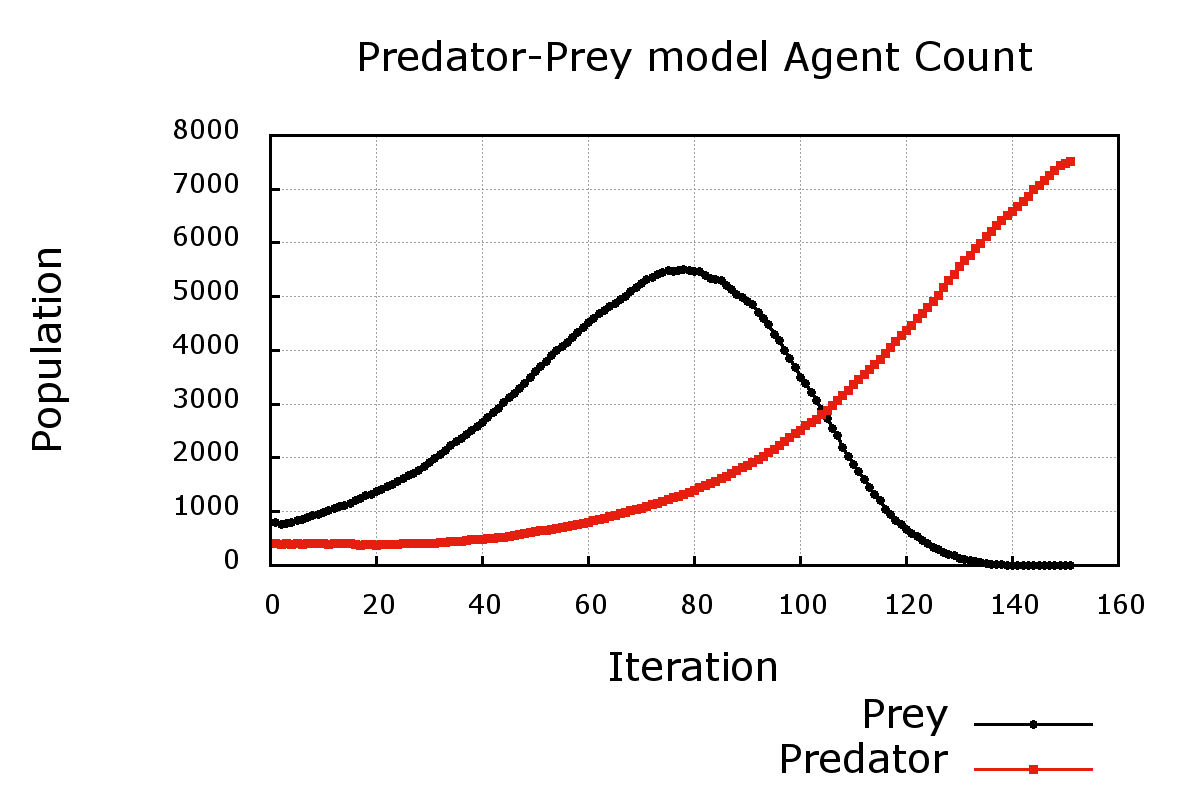
\includegraphics[width=4in]{prey_predator_iter150}
    \caption{Examples of predator-prey model simulation - no grass included (after 150 iteration) }
    \label{fig:simulation_noGrass}
\end{figure}

\section{Exercise 02}
Now, let's change the parameters in the initial data and see how it affects the behaviour. To generate the initial data (0.xml), navigate to \verb|XMLGenerator| folder. 

\begin{enumerate}[{2.1}]
    \item Compile and re-run the executable with different parameters.
%to do
\begin{verbatim} 
cd /examples/PreyPredator/XMLGenerator/
g++ -std=gnu++11 xmlGen.cpp -o xmlGen
./xmlGen ../iterations/0.xml 800 400 0.05 0.03 50
\end{verbatim}
, where 800 is the number of predators, 400 is the number of preys, 0.05 and 0.03 are the reproduction rates for both prey and predator, and 50 is the predator's energy gain. 


\item Re-run the executable again for 300 iterations and plot the results. Your plot should be similar to Figure~\ref{fig:simulation_noGrass_exr2}.

\begin{figure}[!h]
    \centering
    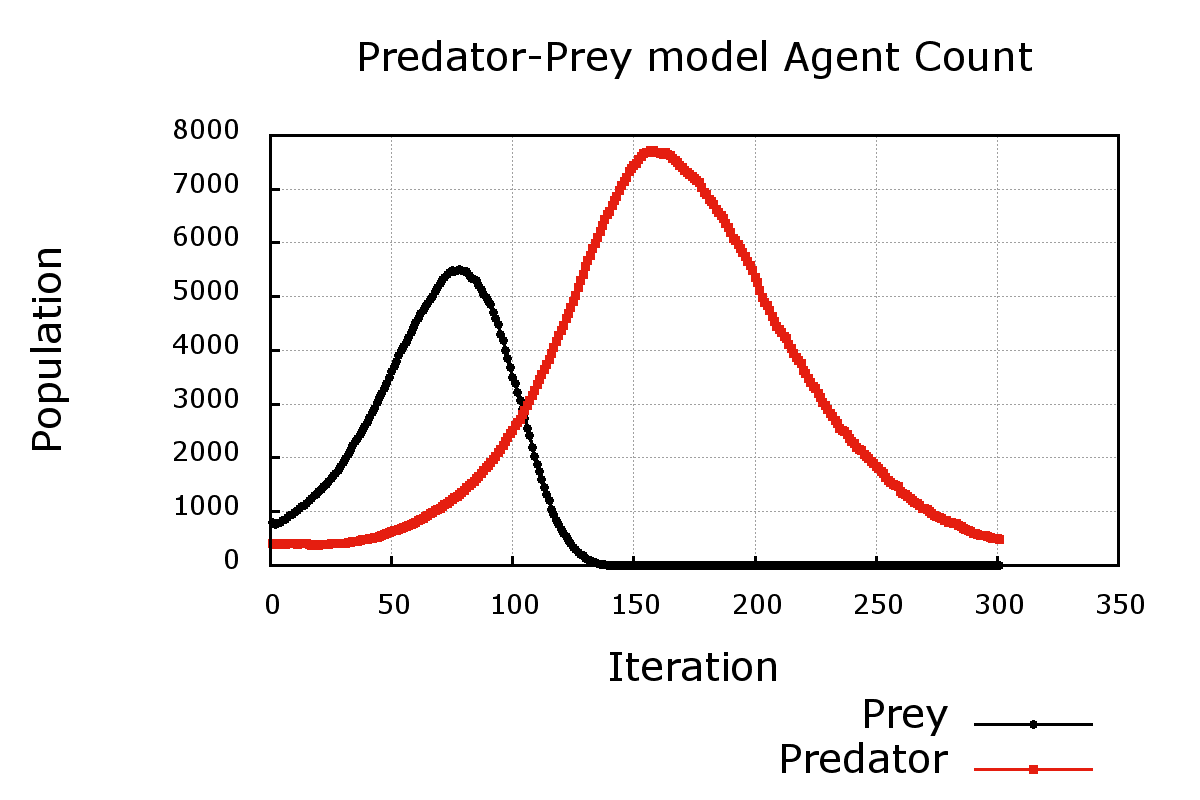
\includegraphics[width=4in]{prey_predator}
    \caption{Examples of predator-prey model simulation - no grass included (after 300 iteration)}
    \label{fig:simulation_noGrass_exr2}
\end{figure}

\item Change the other parameters or the iteration number to see how the behaviour changes.
\end{enumerate}
\section{Exercise 03}
In this exercise, we are going to extend our model to include grass. We have previously described the behaviour of the model when grass included. Agent grass description has already be added to the XML model file. In this exercise, you need to modify \verb|function.c| file to include below functions:

\begin{enumerate}[{3.1}]
\item \textbf{grass\_output\_location}: each grass agent outputs information to be read by other agents
\item \textbf{grass\_eaten}: each grass agent iterates over \verb|prey_location_messages| and checks the distance between its location and the prey agent. If the grass is available and the distances less than \verb|GRASS\_EAT\_DISTANCE|, then the grass is eaten by the closet prey and the regrowth cycle starts. Note that if there are multiple preys within the \verb|GRASS\_EAT\_DISTANCE|, then the closet prey to the grass, eats it and outputs a message \verb|grass_eaten| containing the ID of the prey who ate it.

Once the grass is eaten, its colour changes (\verb|type| variable is set to a different colour) and it no longer will be available until the \verb|death_cycles| reaches \verb|GRASS_REGROW_CYCLES|). 
\item \textbf{prey\_eat\_or\_starve}: each grass agent iterates over \verb|grass_eaten_messages| and checks the ID against it ID. If the grass eaten message indicates that this prey ate some grass then increase the preys life by adding energy. Moreover, if its life is less than 1, it dies.
\item \textbf{grass\_growth}: If the the \verb|death_cycles| variable is equal to \verb|GRASS_REGROW_CYCLES|, then the grass agent becomes available and the \verb|death_cycles| restarts and the colour will be set to green again. If the grass is not available (meaning the \verb|death_cycles| variable is not equal to \verb|GRASS_REGROW_CYCLES|), then we only increase the \verb|death_cycles| variable.
\end{enumerate}


Now, generate a new initial data file using below parameters. Then re-build the model via \verb|make| and run the simulation for 600 iterations \verb|make run_console iter=600|. Your plot should be similar to Figure~\ref{fig:simulation_Grass}.

\begin{verbatim}
cd /examples/PreyPredator/XMLGenerator/
g++ -std=gnu++11 xmlGen_IncGrass.cpp -o xmlGen
./xmlGen ../iterations/0.xml 800 400 2000 0.05 0.03 75 50 100
\end{verbatim}

, where 800 is the number of preys, 400 is the number of predators, 2000 is the number of grass, 0.05 and 0.03 are the reproduction rates for both prey and predator, 75 is the prey's energy gain, and 50 is the predator's energy gain. 


\begin{figure}[!h]
    \centering
    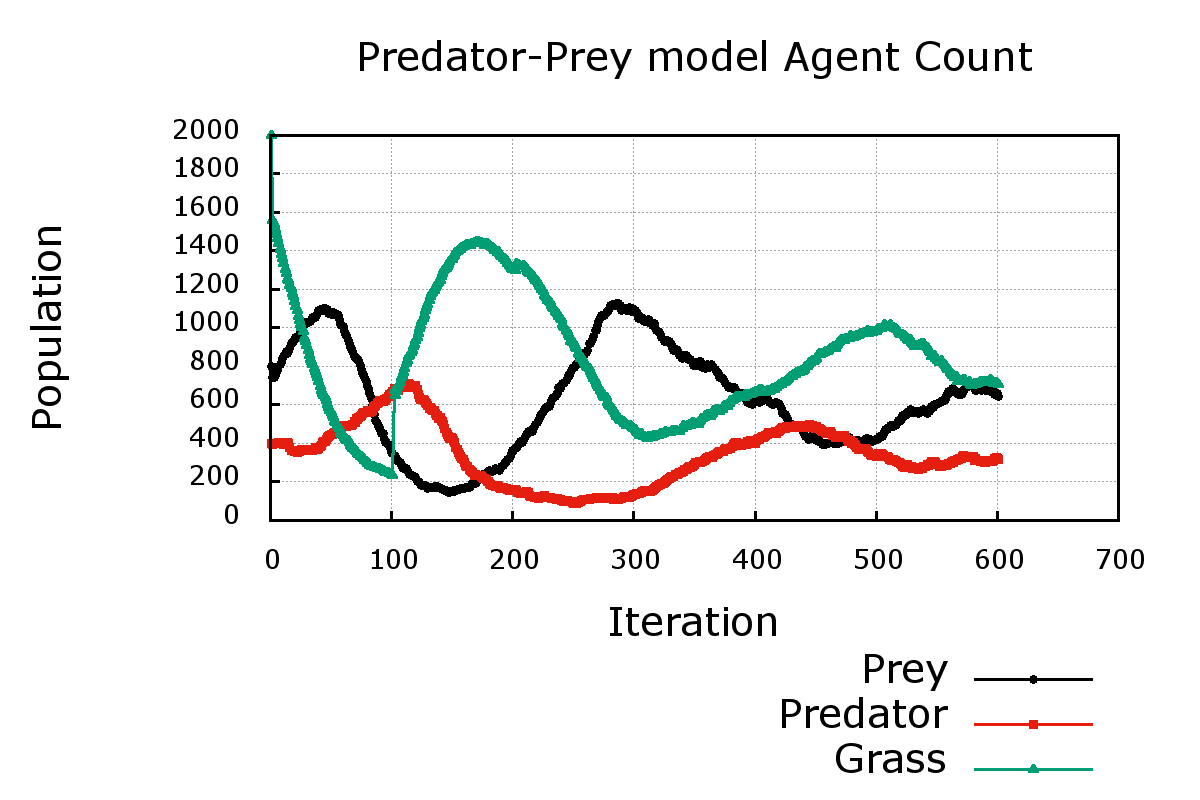
\includegraphics[width=4in]{prey_predator_grass}
    \caption{Examples of predator-prey model simulation with grass included}
    \label{fig:simulation_Grass}
\end{figure}

\section{Experimenting with the Model}
Try changing the parameters to see how this will change the behaviour of the agents causing the behaviours to change.

For more information on FLAMEGPU see the FLAMEGPU website\footnote{www.flamegpu.com} and the documentation which gives detailed instructions on all aspects of FLAMEGPU modelling. More examples can be found on FLAMEGPU GitHub repository (\verb|https://github.com/FLAMEGPU/FLAMEGPU.git|).

You can download the solutions from GitHub (\href{https://github.com/FLAMEGPU/tutorial/}{https://github.com/FLAMEGPU/tutorial/}).


\bibliographystyle{IEEEtran}
\bibliography{bibliography.bib}

\end{document}
